
The total amount spent is given by=

    \begin{multline}
    \vec{B}\vec{A}\\
    =\myvec{1000&500&5000\\3000&1000&10000}\myvec{40\\100\\50}\\
    =\myvec{40000+50000+250000\\120000+100000+500000}\\
    \begin{blockarray}{cc}
    \text{TotalCost} \\
    \begin{block}{(c)(c)}
    340000&\text{X}\\
    720000&\text{Y}\\
    \end{block}
    \end{blockarray}
    \end{multline}
$\therefore$ the total amount spent in city X and city Y is 3400 and 7200 Rupees respectively.  See Fig. \ref{matrix/64fig:Profit}	
%
\begin{figure}[!ht]
\centering
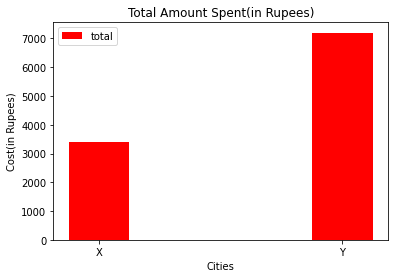
\includegraphics[width=\columnwidth]{solutions/su2021/64/figure8.png}
\caption{Total Amount Spent by the group in cities X and Y}
\label{matrix/64fig:Profit}	
\end{figure}
